% Poisson and Schordinger Solver Flowchart
% Author: Stefan Kottwitz
% The basic procedure of modeling of semiconductor laser diode
% Author: Zhihuan Wang By: 10-10-2016
% https://www.packtpub.com/hardware-and-creative/latex-cookbook
\documentclass[border=20pt]{standalone} 
%%%<
\usepackage{verbatim}
%%%>
\begin{comment}
:Title: Poisson and Schordinger Solver Flowchart
:Tags: Charts;Flowcharts;Cookbook
:Author: Zhihuan Wang
:Slug: laser-flowchart

A flowchart showing how we may choose a math
environment.

It shows using styles, placing nodes in a matrix,
and drawing arrows using loops.
\end{comment}
\usepackage[a4paper,vmargin=3cm]{geometry}
\usepackage{tikz}
\usetikzlibrary{matrix,calc,shapes}
\tikzset{
  treenode/.style = {shape=rectangle, rounded corners,
                     draw, anchor=center,
                     text width=15em, align=center,
                     top color=white, bottom color=blue!20,
                     inner sep=1ex},
  decision/.style = {treenode, diamond, inner sep=0pt},
  root/.style     = {treenode, font=\Large, bottom color=red!30},
  env/.style      = {treenode, font=\ttfamily\normalsize},
  finish/.style   = {root, bottom color=green!40},
  dummy/.style    = {circle,draw}
}
\newcommand{\yes}{edge node [above] {yes}}
\newcommand{\no}{edge  node [left]  {no}}
\begin{document}
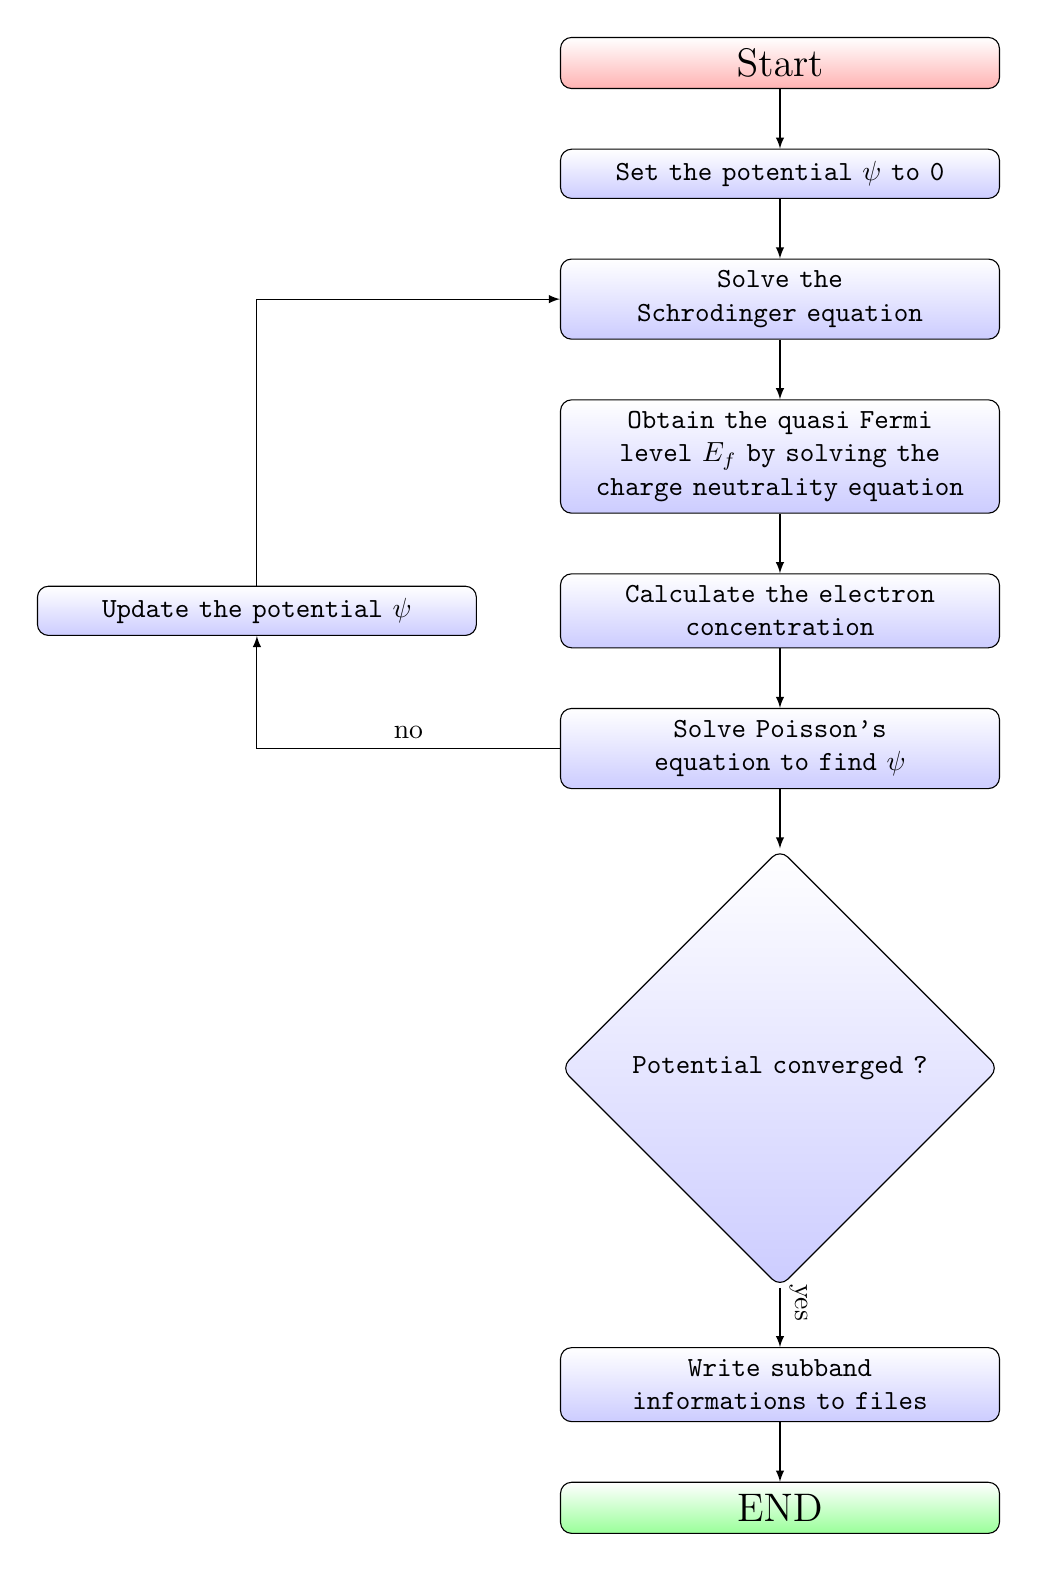
\begin{tikzpicture}[-latex]
  \matrix (chart)
    [
      matrix of nodes,
      column sep      = 3em,
      row sep         = 5ex,
      column 1/.style = {nodes={decision}},
      column 2/.style = {nodes={env}}
    ]
    {
                & |[root]| Start                        \\
                & Set the potential $\psi$ to 0         \\
                & Solve the Schrodinger equation        \\
                & Obtain the quasi Fermi level $E_f$ by solving the charge neutrality equation \\
      |[env]| Update the potential $\psi$         & Calculate the electron concentration    \\
                & Solve Poisson's equation to find $\psi$ \\
                & |[decision]| Potential converged ?      \\
                & Write subband informations to files     \\
                & |[finish]| END        \\
    };

   \draw
     (chart-1-2) edge (chart-2-2)
     (chart-7-2) -- (chart-8-2)
        node[near start,sloped,above] {yes}
     \foreach \x/\y in {2/3, 3/4, 4/5, 5/6, 6/7, 8/9} {
       (chart-\x-2) edge  (chart-\y-2) };
    \draw
      (chart-6-2) -| (chart-5-1)
        node[near start,sloped,above] {no};
    \draw
      (chart-5-1) |- (chart-3-2);
\end{tikzpicture}
\end{document}
